\documentclass[12pt,letterpaper]{article}

\usepackage[brazilian]{babel}
\usepackage[utf8]{inputenc}
\usepackage[T1]{fontenc}

\usepackage{fullpage}
\usepackage{cancel}
\usepackage[top=2cm, bottom=4.5cm, left=2.5cm, right=2.5cm]{geometry}
\usepackage{amsmath,amsthm,amsfonts,amssymb,amscd}
\usepackage{lastpage}
\usepackage{enumerate}
\usepackage{fancyhdr}
\usepackage{mathrsfs}
\usepackage{xcolor}
\usepackage{graphicx}
\usepackage{listings}
\usepackage{hyperref}

\hypersetup{%
	colorlinks=true,
	linkcolor=blue,
	linkbordercolor={0 0 1}
}

\setlength{\parindent}{0.0in}
\setlength{\parskip}{0.05in}

% Edit these as appropriate
\newcommand\course{Rener Oliveira}
\newcommand\lcur{\mathcal{L}}
\newcommand{\real}{\mathbb{R}}
\newcommand{\rr}{\mathbb{R}^2}
\newcommand{\rn}{\mathbb{R}^n}
\newcommand{\linesep}{{\color{black} \rule{\linewidth}{0.5mm} }}
\newcommand{\rpos}{\mathbb{R}_{>0}}
\newcommand{\ex}[1]{\textcolor{blue}{\textbf{Exercício #1}}}
\newcommand{\sol}[1]{\textbf{Solução #1}}
\newcommand{\blue}[1]{{\color{blue}{#1}}}
\newcommand{\bd}[1]{\boldsymbol{#1}}
\pagestyle{fancyplain}
\headheight 35pt        
\chead{\textbf{\Large Lista 4 \\ Curvas e Superfícies}}
\rhead{\small{\course \\ \today}}
\lfoot{}
\cfoot{}
\rfoot{\small\thepage}
\headsep 1.5em

\begin{document}
	\begin{enumerate}
		
		\item [\ex{1}] \textcolor{blue}{Verifique se as seguintes curvas são 2-regulares:}
		\begin{enumerate}[(a)]
			\blue{
			\item $\alpha(t)=(t,t^2,t^3),t\in\real$
			}
			
		Usaremos a definição de \cite{ronaldo}, para curvas 2-regulares, que diz que a curva precisa ser regular e com curvatura estritamente positiva.
		
		Veja que $\alpha'(t)=(1,2t,3t^2)$ que é diferente do vetor nulo, para todo $t$ real por conta da primeira componente  constante igual a $1$. Logo $\alpha$ é regular. Pelo item 7, a curvatura é $\kappa_\alpha(t)=2\sqrt{\dfrac{1+9t^2+9t^4}{(1+4t^2+9t^4)^3}}$, que só seria nula no caso $1+9t^2+9t^4=0$ o que não ocorre, dado que $(9t^2+9t^4)\geq0$ e $1>0$. Logo $\alpha$ é 2-regular.
		
		
		
		\blue{
			\item $\alpha(t)=(t,t^2+2,t^3+t),t\in\real$}
		
		Temos $\alpha'(t)=(1,2t,3t^2+1)$ e $\alpha''(t)=(0,2,6t)$, a velocidade é não-nula pelo termo constante o que faz $\alpha$ ser regular. Usaremos a aceleração no cálculo da curvatura:
		
		\begin{align*}
			\kappa_{\alpha}(t)&=\dfrac{||\alpha''(t)\times\alpha'(t)||}{||\alpha'(t)||^3}\\
			&=\dfrac{||(0,2,6t)\times(1,2t,3t^2+1)||}{||(1,2t,3t^2+1)||^3}\\
			&=\dfrac{||(2-6t^2,6t,-2)||}{(1+4t^2+(3t^2+1)^2)^{3/2}}\\
		\end{align*}
		
		Para evitar contas, dado que queremos analisar se a curvatura é nula ou não, vamos olhar somente o numerador:
		
		\begin{align*}
			||(2-6t^2,6t,-2)||&=\sqrt{(2-6t^2)^2+36t^2+4}\\
			&=\sqrt{4-24t^2+36t^4+36t^2+4}\\
			&=\sqrt{8+12t^2+36t^4}\\
			&\geq0\text{ }\forall t \in \real,\text{ pois } (12t^2+36t^4)\geq0\text{ e } 8>0
		\end{align*}
		
		Com isso, concluímos que $\alpha$ é 2-regular.
	\end{enumerate}

	\item[\ex{2}] \textcolor{blue}{Prove que a aplicação $\alpha(t) = (1 +\cos(t),\sin(t),2\sin(t/2),t\in\real$, é uma curva regular cujo traço está contido na interseção do cilindro $C= (x,y,z)\in\real^3; ~(x-1)^2+y^2= 1$ e da esfera $S= (x,y,z)\in\real^3;~x^2+y^2+z^2= 4$. Desenhe a curva $\alpha$, o cilindro $C$ e a esfera $S$ em ambiente computacional}
	
	\item[\sol{2}] A duas primeiras coordenadas da velocidade, a menos de sinal, são $\sin (t)$ e $\cos(t)$ que já foi provado no início da \href{https://github.com/reneroliveira/Curves_and_Surfaces/blob/main/lists/list3.pdf}{Lista 3} que não serão ao mesmo tempo. A terceira componente é, à menos de constantes $\cos(t/2)$. É fácil ver que ela não zera quando $\cos(t)=0$; O único problema seria com ângulos $t=\pi+2k\pi$, onde $\sin(t)=\cos(t/2)=0$, mas neste caso a componente $\cos(t)\neq0$. Podemos então assegurar que as componentes não se anulam ao memso tempo, comprovando a regularidade da curva.
	
	\begin{figure}[!htb]
		\centering
		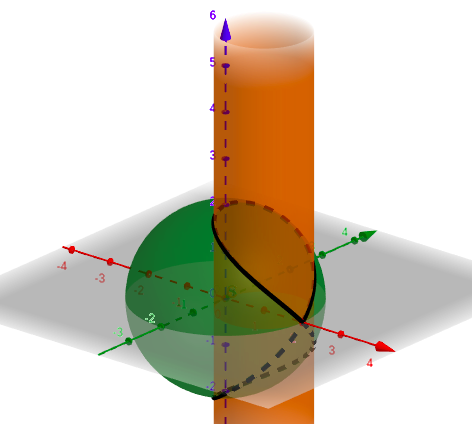
\includegraphics[scale=0.7]{../images/L4_ex2.png}
		\caption{Catetária sob o intervalo (-3,3)}
		\label{ex3}
	\end{figure}
	\item[\ex{3}] \textcolor{blue}{Obtenha uma reparametrização por comprimento de arco da curva }
	\blue{
	$$\alpha(t)=(e^t\cos(t),e^t\sin(t),e^t),~t\in\real$$}
	\item[\sol{3}] Encontrando a função comprimento de arco:
	
	\begin{align*}
		\lcur(t)&=\int_{t_0}^{t}||\alpha'(u)||du\\
		&=\int_{t_0}^{t}||e^u(-\sin u,\cos u,1)||du\\
		&=\int_{t_0}^{t}e^u(\sin^2u+\cos^2u+1)^{1/2}du\\
		&=\sqrt2\int_{t_0}^{t}e^udu\\
		&=\sqrt2(e^t-e^{t_0})
	\end{align*}
		
		Tomando os devidos cuidados com os domínios e imagens, podemos inverter a função comprimeiro de arco, fixando  gerando $\lcur^{-1}(t)=\ln\left(\dfrac{t}{\sqrt2}+e^{t_0}\right)$
		
		Assim, tomando $s_t=\dfrac{t}{\sqrt2}+e^{t_0}$ a reparametrização por comprimeiro de arco será:
		
		\begin{align*}
			\alpha(\lcur^{-1}(t))&=s_t\left(\cos\left(s_t\right),\sin\left(s_t\right),1\right),
		\end{align*}
	
	Onde está definida para valores de $t$ na qual $\dfrac{t}{\sqrt2}+e^{t_0}>0\Rightarrow t>-e^{t_0}\sqrt2$.
	
	\item[\ex{7}] \textcolor{blue}{Calcule a curvatura e a torção das seguintes curvas:}
		\begin{enumerate}[(a)]
			\blue{
			\item $\alpha(t)=(t,t^2,t^3),t\in\real$}
				\begin{align*}
					\kappa_{\alpha}(t)&=\dfrac{||\alpha''(t)\times\alpha'(t)||}{||\alpha'(t)||^3}
					=\dfrac{||(0,2,6t)\times(1,2t,3t^2)||}{||(1,2t,3t^2)||^3}\\
					&=\dfrac{||(-6 t^2, 6 t, -2)||}{(1+4t^2+9t^4)^{3/2}}
					=\dfrac{2||(-3t^2,3t,-1)||}{(1+4t^2+9t^4)^{3/2}}\\
					&=\dfrac{2(1+9t^2+9t^4)^{1/2}}{(1+4t^2+9t^4)^{3/2}}\\
					&=2\sqrt{\dfrac{1+9t^2+9t^4}{(1+4t^2+9t^4)^3}}
				\end{align*}
			
			
			
			\begin{align*}
				\tau_\alpha(t)&=\dfrac{\langle(\alpha'(t)\times\alpha''(t)),\alpha'''(t)\rangle}{||\alpha'(t)\times\alpha''(t)||^2}\\
				&=\dfrac{\langle(6 t^2, -6 t, 2),(0,0,6)\rangle}{||(6 t^2, -6 t, 2)||^2}\\
				&=\dfrac{12}{36t^4+36t^2+4}\\
				&=\dfrac{3}{9t^4+9t^2+1}
			\end{align*}
		
		\blue{\item $\beta(t)=(\cos t,\sin t,t),t\in\real$}
		
		Como $||\beta'(t)||=||(-\sin t,\cos t,1)||=\sqrt2$ a curva $\beta$ não é unit-speed, podemos reparametrizar por comprimento de arco, trnasformá-la em unit-speed e calcular a curvatura e torção a partir daí. 
		
		É fácil ver que fazendo $t_0=0$, $\lcur_\beta(t)=\sqrt2t$, logo $\lcur^{-1}_\beta(t)=t/\sqrt2$, e a cruva reparametrizada será:
		
		$$\beta(t)=(\cos(t/\sqrt2),\sin(t/\sqrt2),t/\sqrt2)$$
		\begin{align*}
			\kappa_{\beta}(t)&=||\beta''(t)||\\
			&=\dfrac{1}{\sqrt2}||(-\sin (t/\sqrt2),\cos (t/\sqrt2),1/\sqrt2)'||\\
			&=\dfrac{1}{2}||(-\cos (t/\sqrt2),-\sin (t/\sqrt2),0)||\\
			&=\dfrac{1}{2}\sqrt{\sin^2(t/\sqrt2)+\cos^2(t/\sqrt2)}\\
			&=\dfrac{1}{2}
		\end{align*}
		
		Para a torção, vamos determinar os vetores tangente (T), normal (N) e binormal (B), do Triedro de Frenet, e calcular torção como a $\tau(s)$ tal que $B'(s)=\tau(s)N(s)$.
		
		\begin{align*}
			T(s)&=\dfrac{1}{\sqrt2}(-\sin (s/\sqrt2),\cos (s/\sqrt2),1)\\
			N(s)&=(-\cos (s/\sqrt2),-\sin (s/\sqrt2),0)\\
			B(s)&=T(s)\times N(s)\\&=\dfrac{1}{\sqrt2}(\sin(s/\sqrt2),-\cos(s/\sqrt2),1)
		\end{align*}
		\end{enumerate}
	
		
	\end{enumerate}
	\newpage

% \addcontentsline{toc}{section}{Referências}
\bibliographystyle{plain}
\bibliography{refs}
\end{document}